%2345678901234567890123456789012345678901234567890123456789012345678901234567890
%%%%%%%%%%%%%%%%%%%%%%%%%%%%%%%%%%%%%%%%%%%%%%%%%%%%%%%%%%%%%%%%%%%%%%%%%%%%%%%%
% MAURICIO ESGUERRA NEIRA
% Ph. D. Thesis
%%%%%%%%%%%%%%%%%%%%%%%%%%%%%%%%%%%%%%%%%%%%%%%%%%%%%%%%%%%%%%%%%%%%%%%%%%%%%%%%
\chapter{RNA Base Steps}
\label{basesteps} 
\bibliographystyle{nar}
The problem of classification of the space of conformations
%configurations?
of RNA  is not  new, see for  example, Olson  1972 \cite{olson1_1972},
Saenger     1984     \cite{saenger1984},     and    Gautheret     1993
\cite{gautheret1993}.  Although only  a few researchers addressed this
problem  before  the  turn  of  the twenty  first  century,  now  this
situation is changing rapidly. The reason for this fast change came in
the year 2000, when a vast amount of RNA structural information became
available  upon the  elucidation of  the  structure of  the 30S  small
ribosomal  subunit  of   \textit{Thermus  thermophilus},  a  bacterial
ribosome  \cite{wimberly2000,  schluenzen2000},   and  the  50S  large
ribosomal subunit of \textit{Haloarcula marismortui}, an archaeal
%\footnote{I emphasize the  phylogeny of rRNA's here since  there is an
%  ongoing discussion among biologists on whether archaea are closer to
%  prokaryotes, or to eukaryotes.}
ribosome \cite{ban2000}.
\begin{figure}[H]
\centering
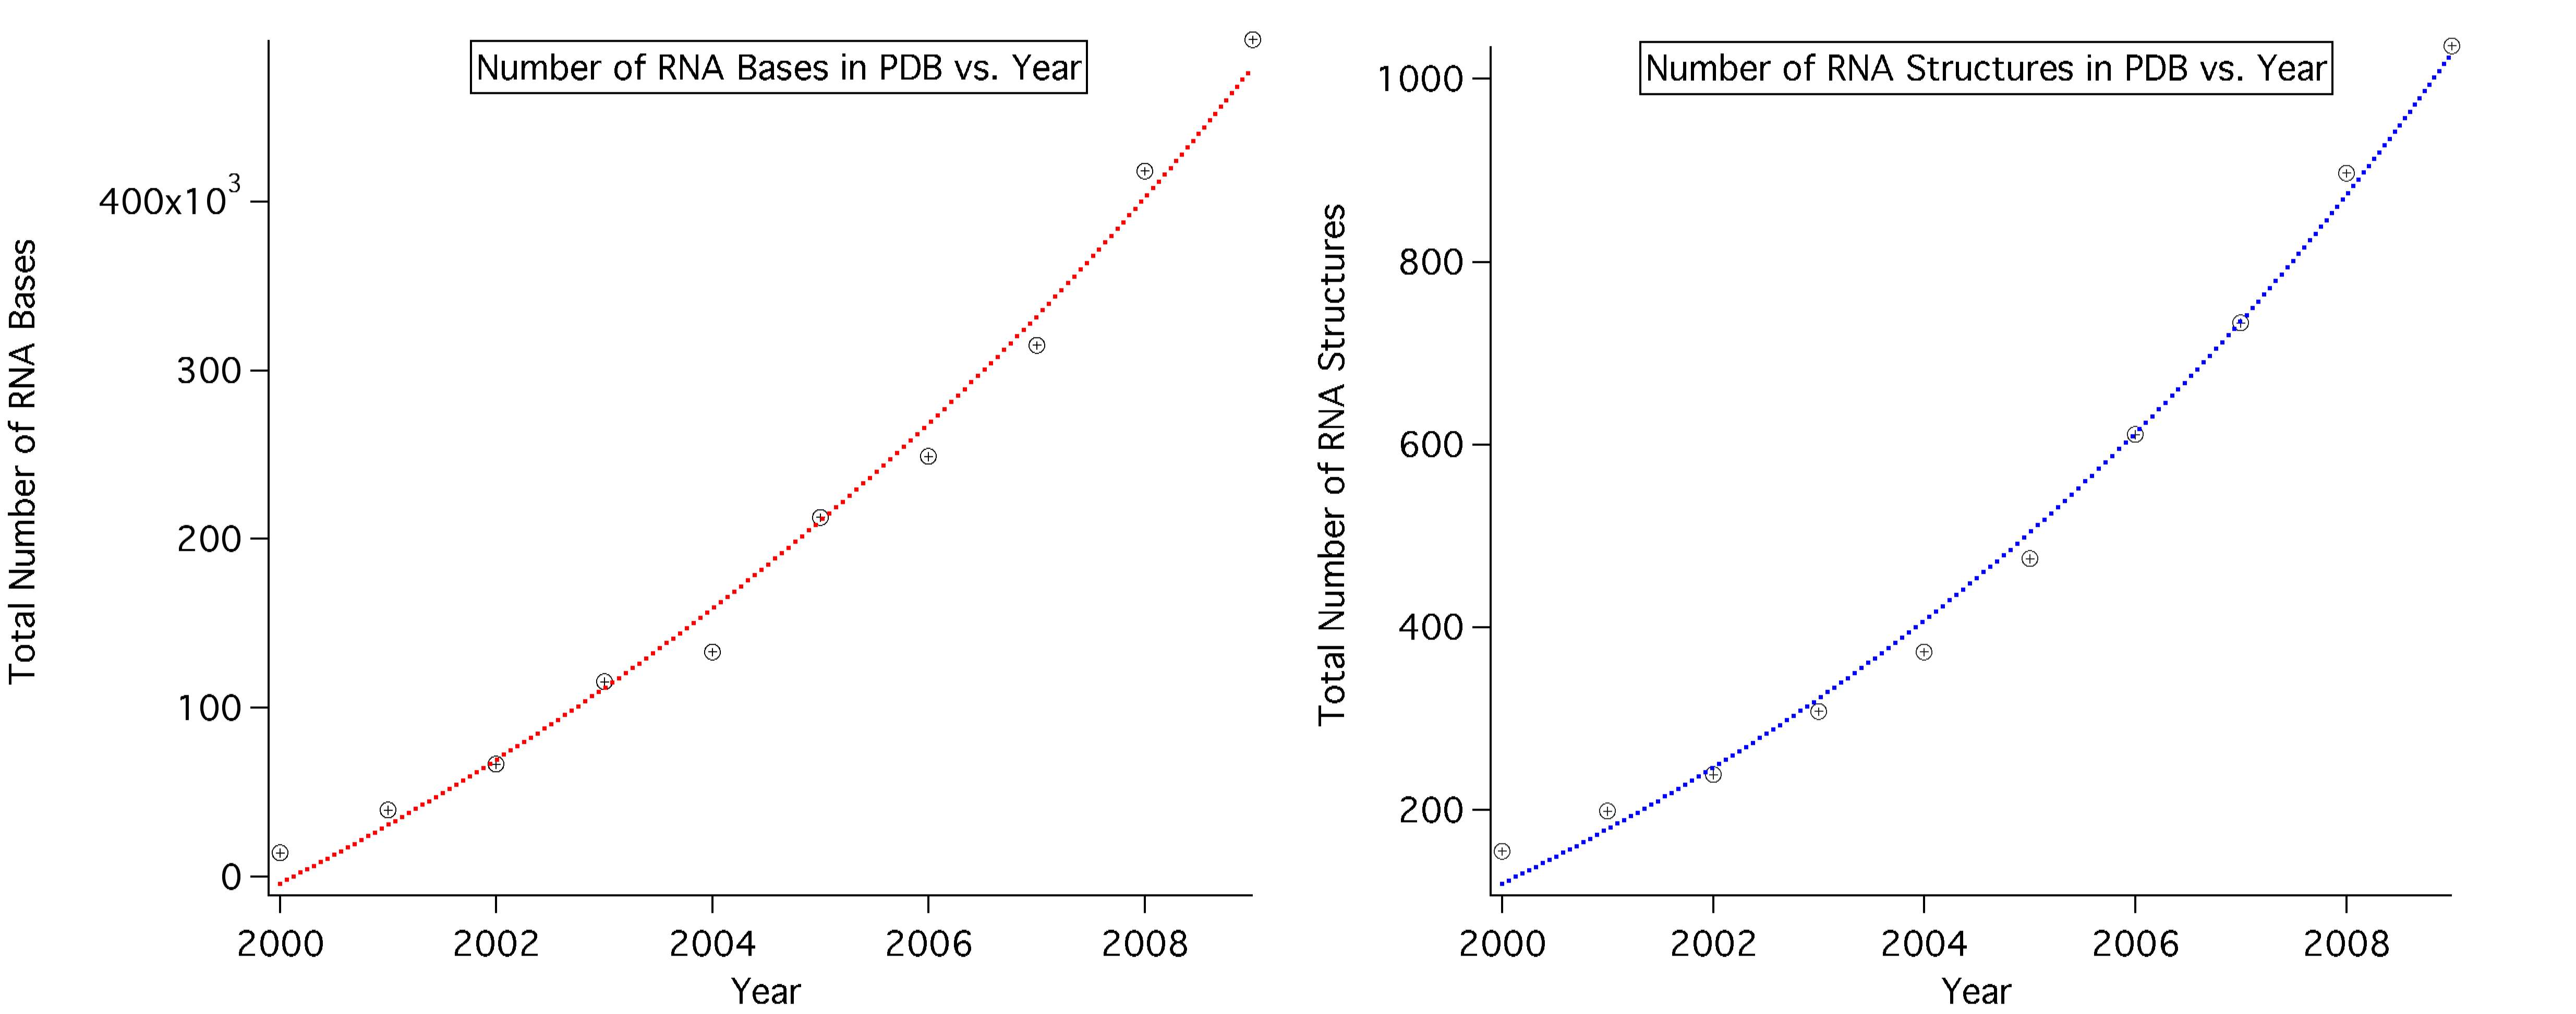
\includegraphics[scale=0.38]{Chapter2/rna2000_2009copy.png}
\caption{\textbf{Left:} Total number of RNA bases added to the Protein
Data Bank (PDB)  database between 2000 and 2010  (exponential fit line
in blue). \textbf{Right:} Total number of RNA structures solved yearly
by X-ray  crystallography between 2000 and 2010  (exponential fit line
in red).}
\label{fig:rnainpdb}
\end{figure}

\noindent Between  1978 and  2000 a total  of 116 RNA  structures with
resolution better than 3.5  \AA, and comprising around 5500 nucleotide
bases were added to the Protein  Data Bank (PDB), and between 2000 and
today  931  RNA\index{RNA}  structures  comprising  491158  nucleotide
bases.  That  is, the increase in  information due to  the solution of
large  RNA structures as  pointed out  by Noller  \cite{noller2005} is
about two  orders of  magnitude. It  is clear from  the growth  of RNA
structural  information from  2000  until today  that  both the  total
number of RNA structures deposited in the PDB, and the total number of
nucleotide bases in these  structures, is increasing at an exponential
rate  (as can  be seen  from  the exponential  fits of  these data  in
Figure~\ref{fig:rnainpdb}).  It is important  to note that such growth
comes mainly from ribosomal structures which contain 88 percent of all
RNA bases in  the PDB.  So, even though structural  interest in RNA is
growing  since  ribosomal structures  became  available  in 2000,  and
several Nobel prizes  have been awarded for work  in this field, along
with   the   exciting   possibilities   of   deciphering   large   RNA
\cite{weinberg2009}  structures  other than  the  ribosome, still  the
growth of  the RNA structural  field is far  from that of  proteins if
weighed by  the growth in  diversity of RNA structural  information in
the past decade.  If we look  at the current distribution of the sizes
of  RNA   structures  counted  in   terms  of  the  number   of  bases
(Figure~\ref{fig:rnaranges}) it is clear  that there are large patches
where there are  no RNA structures whatsoever.  That  is, there are no
solved structures  of RNA with  roughly 600 to  1400 bases or  1800 to
2700  bases.  The  area of  non-coding RNA's  holds great  promise for
finding structured RNA's  in such length ranges, as  has recently been
suggested by Breaker \cite{weinberg2009}.  A representative example of
the characteristic ranges  of RNA structures available to  date in the
PDB can be seen in Table~\ref{tab:rnarange} for structures larger than
300  bases. A  comparison between  the total  number of  structures of
protein, protein plus nucleic acid, DNA, and RNA, available at the PDB
from   the  seventies   until  today   can  be   seen   in  Supplement
Figure~\ref{fig:allpolypdb}.  The most  notable feature of this figure
is  the  large difference  between  the  number  of deposited  protein
structures and  nucleic acid structures, which have  to be represented
with an offset  of an order of magnitude in  number of structures. The
other prominent feature is that of the difference in growth of DNA vs.
RNA structural information. RNA structures seem to be growing steadily
since the mid-nineties, whereas DNA structural information seems to be
tending to a constant number, or having a very small growth.
\begin{figure}
\centering
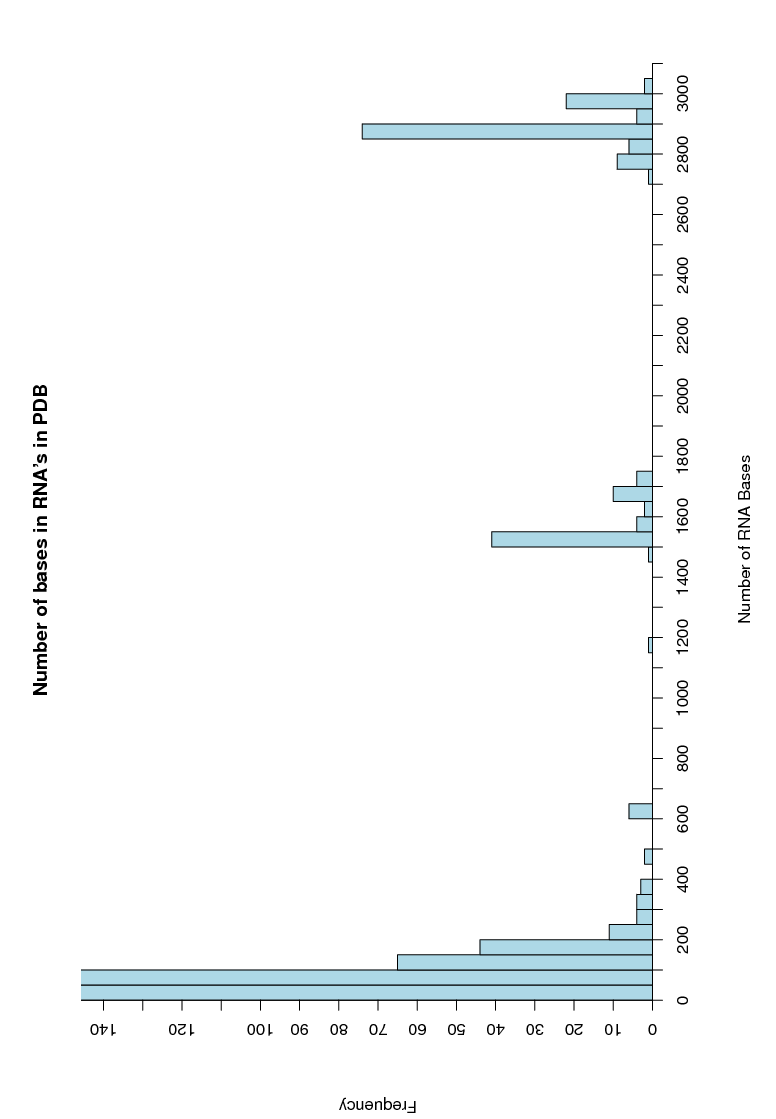
\includegraphics[scale=0.60, angle=270]{Chapter2/histogram.png}
\caption{Frequency of  nucleotide bases in RNA molecules  found in the
  PDB classified by  the size of RNA molecules. We  define the size as
  the total number of nucleotide bases present per molecule.}
  \label{fig:rnaranges}
\end{figure}
%The table and Figure 1.1 come from downloading all structures from
%2000, until today that have RNA in the pdb and that have a resolution
%better that 3.0A, they are 460 structures.

\noindent The analysis of  the conformational information contained in
RNA  structures  can  be  divided  into three  main  perspectives:  an
atom-based perspective; a bond-based  perspective; and a third, as yet
unexplored  to our  knowledge, rigid-body-based  perspective.   In the
atom-based perspective,  either a  direct comparison of  backbone atom
positions  is  made  \cite{reijmers2001},   or  a  comparison  of  the
distances between  a reduced  set of atoms  taken from  the nucleotide
backbone, sugar,  and base  \cite{sykes2005} is made.   The bond-based
perspective  is  divided  into   three  main  categories.   The  first
considers the consecutive  covalent bonds in the RNA  backbone and the
glycosidic  bond between  the sugar  and base,  that is,  six backbone
torsion  angles and one  glycosidic torsion  angle \cite{reijmers2001,
murray2003,  hershkovitz2003,  schneider2004,  hershkovitz2006}.   The
second   considers  the   pseudo-bonds  between   consecutive   P  and
C4$^{\rm{\prime}}$  atoms  and  the  resulting  pseudo-torsion  angles
$\eta$   and  $\theta$   \cite{olson1_1972,   duarte1998,  duarte2003,
wadley2007} \footnote{Previously  the pseudotorsion angles  $\eta$ and
$\theta$     were    given     the    names     $\omega_{\nu}$,    and
$\omega_{\nu'}$.\cite{olson1980,  malathi1985}}.   The third  category
considers the networks of  horizontal hydrogen bonding patterns coming
from  a definition of  interacting edge  boundaries in  the nucleotide
bases \cite{westhof2000, leontis2002, leontis2006}. In this chapter we
study the  rigid-body based perspective using  clustering analysis and
discuss  the  relationship  of  these  findings  to  other  previously
reported perspectives on RNA conformation.
\begin{table}[htbp]
\begin{center}
{\small
\begin{tabular}{c|p{5cm}|c|c|c}
\hline
\bf{PDBID} & \bf{Structure Name} & \bf{Phylogenetic Group} & \bf{Number of bases} & \bf{Year} \\ \hline
1l8v & Mutant of P4-P6 Domain of Group I Intron & Eukaryote & 314 & 2002 \\ \hline
3igi & Group II Intron & Bacteria & 395 & 2009 \\ \hline
1fg0 & Central Loop in Domain V of 23S rRNA & Archaea & 499 & 2000 \\ \hline
2nz4 & GlmS Ribozyme & Eukaryote & 604 & 2006 \\ \hline
1xmq & 30S rRNA & Bacteria & 1522 & 2004 \\ \hline
1ffk & 50S rRNA Subunit & Archaea & 2828 & 2000 \\ \hline
\end{tabular}
}
\caption{Some large  RNA structures  ($>$300 bases) elucidated  in the
  last decade.}
\end{center}
\label{tab:rnarange}
\end{table}

\section{Consensus Clustering of Single Stranded Base Step Parameters}
To  our  knowledge there  has  been  no  classification of  rigid-body
base-step parameters for the RNA  structures now available in the PDB.
It is important to note here that in crystal structures, the RNA bases
are determined  more accurately than  the backbone torsion  angles, as
has been  shown by Richardson  and collaborators from the  analysis of
van  der Waals  steric  clashes.  This  can  be seen  more clearly  in
Figure~\ref{fig:murray},    reproduced    from    Richardson's    work
\cite{murray2003}, where the red and orange dots in the backbone atoms
region denote steric clashes and the green and yellow dots in the base
atoms region  denote very good  agreement with expected van  der Waals
distances.
\begin{figure}[htbp]
 \centering
 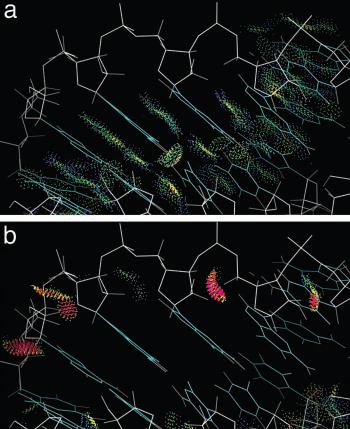
\includegraphics[scale=0.5]{Chapter2/murray2003.png}
 \caption{Comparison of base vs.  backbone structure in RNA reproduced
with permission from Jane  Richardson \cite{murray2003}. Here the blue
and green  dots in (a) denote  very accurate van  der Waals distances,
and the  red and orange  dots on (b)  denote steric clashes,  that is,
distances outside the acceptable van der Waals range.}
 \label{fig:murray}
\end{figure}

\subsection{Combining Fourier Averaging Results and Clustering Analysis}
We   used   standard   clustering   analysis  (CA)   techniques   (see
Appendix~\ref{appendix_a}) to classify  the non-ARNA base-steps in the
coordinate files of 20 rRNA  structures grouped in torsion angle space
by  Schneider  at  al.\cite{schneider2004}.  Here  we  describe  these
structures in terms of the  base-step parameters space. That is, three
translational parameters  (Shift $D_x$, Slide $D_y$,  Rise $D_z$), and
three   rotational  parameters  (Tilt   $\tau$,  Roll   $\rho$,  Twist
$\omega$), in the hexaparametric vector $\nu$:
\begin{gather}
\nu = (D_x, D_y, D_z, \tau, \rho, \omega)
\end{gather}
The    results    illustrated    in    the   dendrogram    shown    in
Figure~\ref{fig:eucl_cons}  were  obtained  by  performing  clustering
analysis  and  consensus  clustering  on  20  structures  provided  by
Schneider et al.   \cite{schneider2004}. These twenty structures which
are  illustrated  in Figures~\ref{fig:nonAclus}  and~\ref{fig:steps2},
were  obtained by  Schneider et  al. by  applying a  Fourier averaging
technique and  lexicographical clustering to the  torsion angles found
in the large subunit of ribosomal RNA (PDB\_ID:1jj2).  The methodology
we used follows  the approach taken by others  to recover the Periodic
Table  classification of the  elements from  multidimensional property
vectors of the elements \cite{restrepo2004, restrepo2006}.
\begin{figure}[htbp]
 \centering
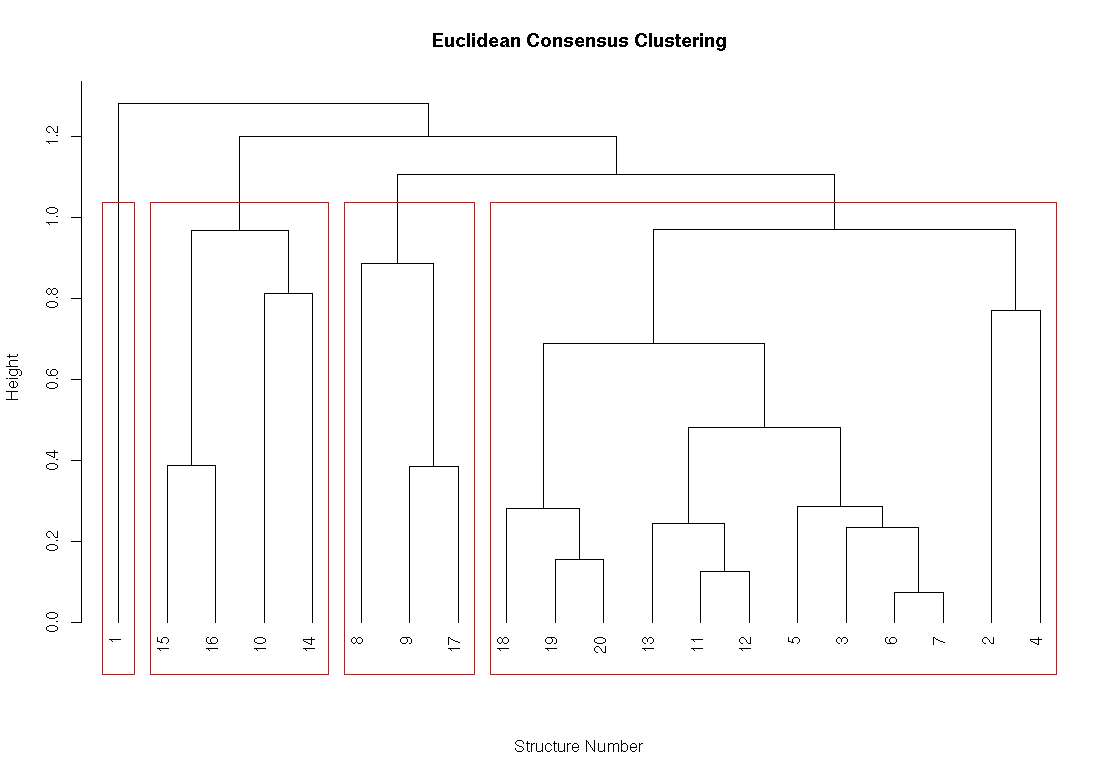
\includegraphics[angle=90, scale=0.6]{Chapter2/eucli_cons_nonA-RNA.png}
\caption{Dendrogram showing the results  of consensus clustering of 20
non-A-type  rRNA  dinucleotides   according  to  their  hexadimensional
base-step parameter vectors.}
 \label{fig:eucl_cons}
\end{figure}

\begin{figure}[htbp]
 \centering
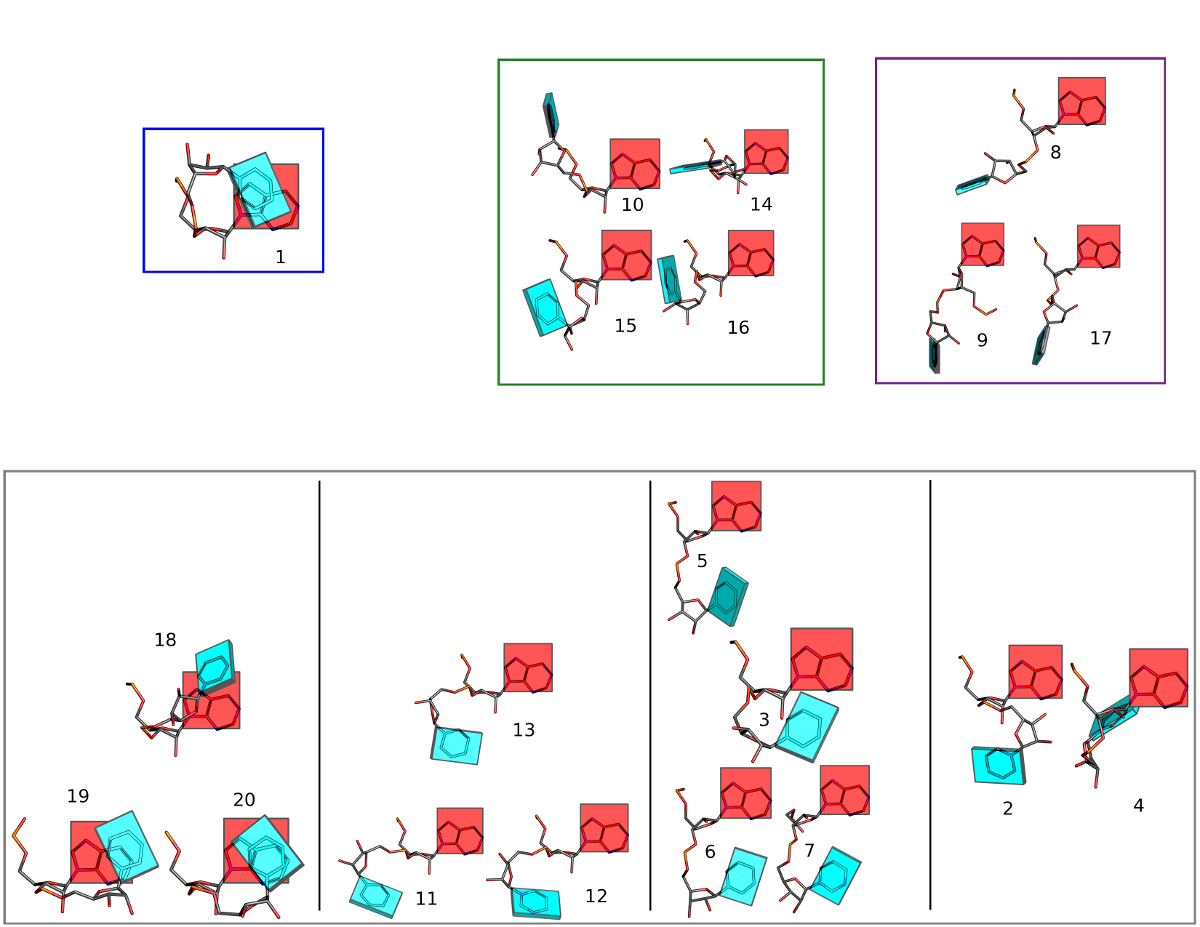
\includegraphics[angle=90, scale=0.46]{Chapter2/collageb.png}
 \caption{non-A-RNA  dinucleotide  structures  organized  by  clusters
   obtained  from   consensus  clustering  of   their  hexadimensional
   base-step parameter vectors.  The  structures have been centered on
   the reference frame  of the first step, that  is, the adenine base,
   with the minor groove edge of the rigid block on adenine facing the
   viewer.}
 \label{fig:nonAclus}
\end{figure}

As is clear  from figures~\ref{fig:nonAclus} and~\ref{fig:steps2}, the
20 identified by Schneider et  al. fall into seven unique groups based
in  the  relative position  of  base  side  groups. Group  I  contains
structure {1}  with bases stacked  and base-plane normals  pointing in
opposite   directions,   Group    II   includes   extended   unstacked
conformations  with neighboring  bases widely  displaced  and oriented
roughly perpendicular  to each other  in all cases --  structures {15,
  16, 10, 14}, Group III also contains extended conformations but with
the uracil on the minor-groove edge of adenine the bases perpendicular
to one another the uracil lies  in the "C8-carbon" of adenine in these
cases -- structures {8, 9, 17}. The bases in each of the conformers in
Group IV  are moer parallel to  one another but are  displaced in four
different  ways.   The bases  in  Group IV  a  structures  {2, 4}  are
unstacked and neither parallel nor  perpendicular. Those in Group IV b
-- structures {18, 19, 20} are  closely related to A-RNA with parallel
and stacked  bases. The bases in  group IV c, structures  {11, 12, 13}
are parallel  but unstacked  with uracil on  the major-groove  edge of
adenine. The bases  on IV d structures {3, 5, 6,  7} are also parallel
and unstacked but  with the long axis of  uracil perpendicular to that
of adenine.  As is clear from figure~\ref{fig:nonAclus} the conformers
in subgroups IV (c) and IV  (d) are closely related, and the dimers in
these two subgroups  are more closely related to  those in subgroup IV
(b) than to those in subgroup IV (a).

In order  to map back into the  23 subunit of the  ribosome the groups
which   were   obtained   by   clustering   we   have   computed   the
root-mean-square deviation (RMSD)  between the average normalized step
parameters of the  structures composing each of the  seven groups, and
the   normalized  \footnote{For  details   on  the   normalization  of
  step-parameters see Equation~\ref{eq:normalization}} step-parameters of the
2753 steps present  in the 23S subunit of  the large ribosomal subunit
(PDB\_ID:1jj2).  That  is, for  each group we  have obtained a  set of
RMSD  values  which  have  been  plotted as  histograms  as  shown  in
Figures~\ref{fig:histo1}, and~\ref{fig:histo2}.

The results are also  summarized in Table~\ref{tab:nonA}, where we can
see that they only constitute 31\% of the total amount of steps in the
23S subunit of the ribosome.  We  used a cutoff of 10 \AA \footnote{We
  retain the  traditional unit of  Angstroms to refers to  our RMSD's,
  but it  is important to  note that since  we are not refering  to an
  all-atom model such  unit does not have a  direct physical meaning.}
to select the  structures which belong to each  group, based on visual
analysis  of superimposed reconstructed  structures. For  example, for
Group I; if we reconstruct the ribosomal steps with an RMSD of 10 \AA~
or   less,  we   get  the   figure  shown   in  the   left   panel  of
Figure~\ref{fig:superimpose}. But  if we  reconstruct with the  set of
structures  with  an  RMSD  of  15  \AA~  or  less  we  start  getting
structures,  which after  being  superimposed based  on the  reference
frames of the first base are clearly not related to that group, as can
be seen in the right panel of Figure~\ref{fig:superimpose}.

We find  that the  A-RNA starting structure  kindly provided to  us by
Schneider et al. differ from canonical A-RNA in that the rise value is
4.39 \AA, rather than the  3.30 \AA~ standard value obtained for A-RNA
by Arnott and collaborators  \cite{arnott1973}. This might have affect
on the number of structures which  can be grouped under the A-RNA like
group.

Because of not getting a good representation of the total diversity of
base-steps  in the  23S  subunit of  the  ribosome, we  have opted  to
perform an  analysis based fully  on base-step parameters.  We believe
that the reason  for such poor representation is due  to the mixing of
Fourier averaging for backbones, and  the base-step perspective.
%% or it could also be  related to the fact that we  are ignoring the
%% remaining A-RNA related set of structures in Berman and
%% collaborators analysis.

\begin{table}[htbp]
\begin{center}
{\footnotesize
\begin{tabular}{c|r|c}
\hline
\bf{Group} & \bf{Percentage} & \bf{Number of Base-Steps}\\ \hline
I   & 0.11  & 3   \\ \hline
II  & 0.18  & 5  \\ \hline
III & 0.04  & 1  \\ \hline
IVa & 0.36  & 1  \\ \hline
IVb & 29.31 & 807 \\ \hline
IVc & 0.33  & 9  \\ \hline
IVd & 1.27  & 35 \\ \hline \hline
Total & 31.28 & 861   \\ \hline
\end{tabular}
}
\caption{Number of base-steps  with RMSD values less than  or equal to
  10 \AA ~between the reference  base-step vectors from the four groups
  of  non-A-type  RNA  dinucleotide  conformations and  all  base-step
  vectors found in the  23S strand of \textit{Haloarcula marismortui}.
  The  percentage  is calculated  with  respect  to  a total  of  2753
  base-steps  present in  the  23S chain  of  the 50S  subunit of  the
  ribosome.}
\label{tab:nonA}
\end{center}
\end{table}

\begin{figure}[htbp]
 \centering
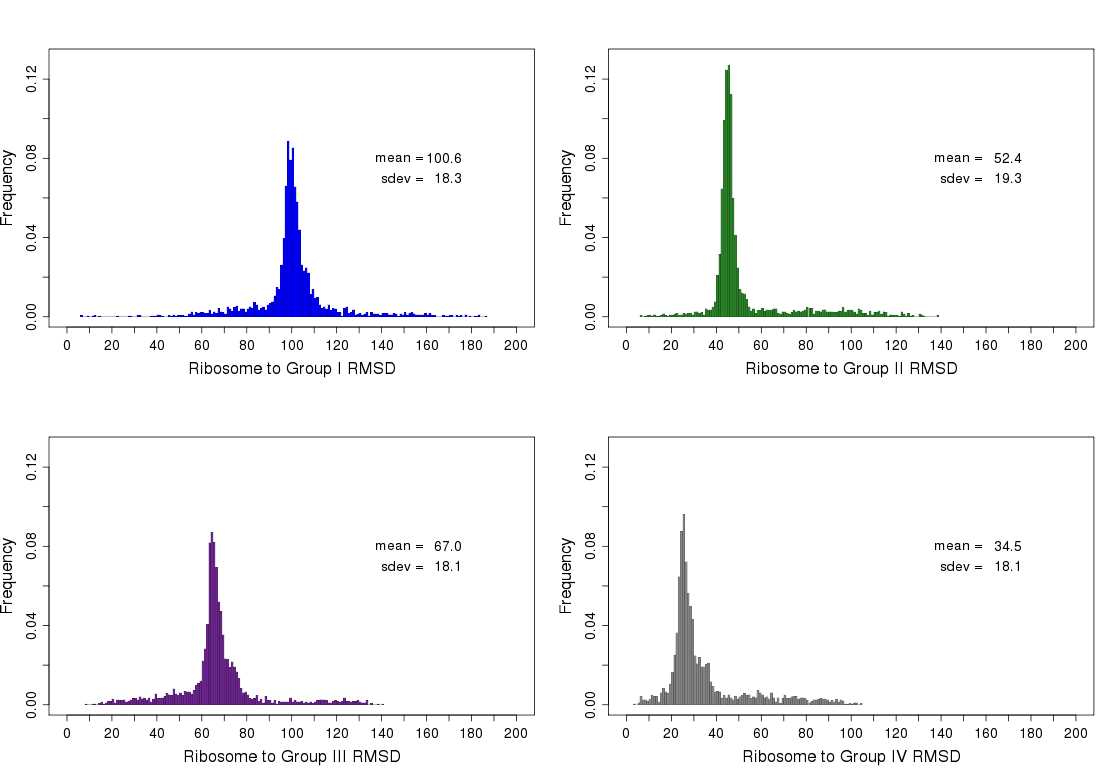
\includegraphics[angle=90, scale=0.6]{Chapter2/RMSDschneider1.png}
\caption{Root mean square deviation of the main four groups show in
  Figure~\ref{fig:nonAclus}. The color of the histograms is the same
  as that of the boxes surrounding the structures of
  Figure~\ref{fig:nonAclus}}
 \label{fig:histo1}
\end{figure}

\begin{figure}[htbp]
 \centering
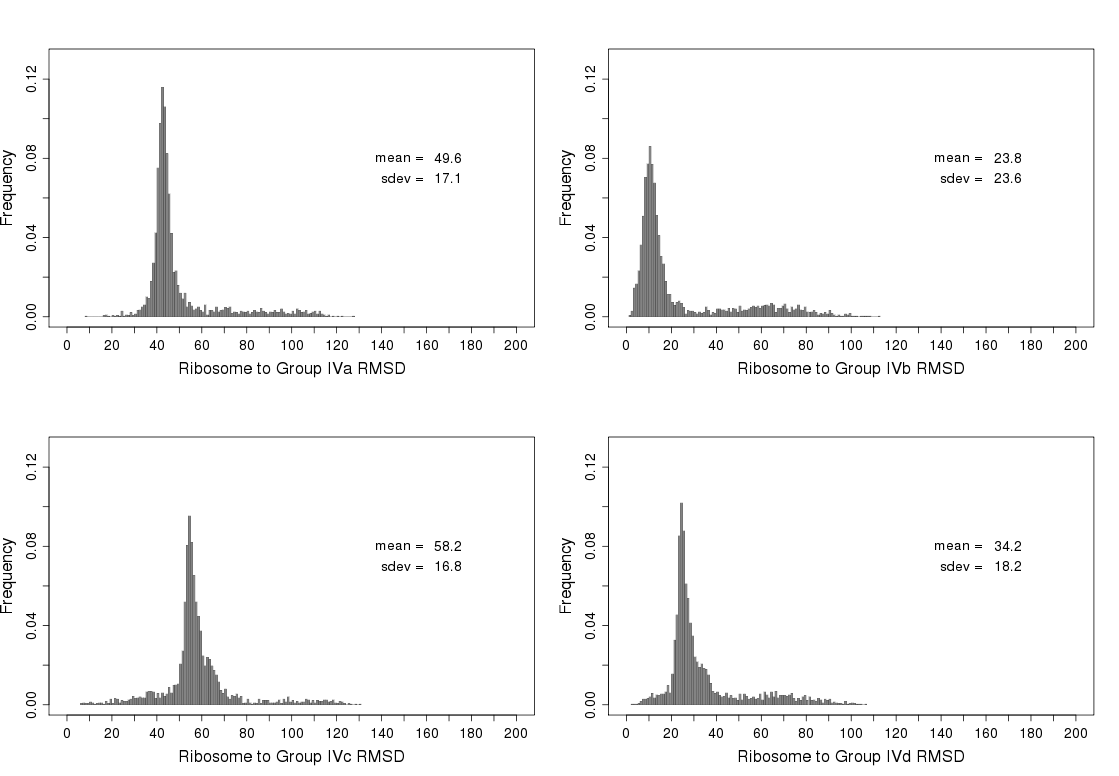
\includegraphics[angle=90, scale=0.6]{Chapter2/RMSDschneider2.png}
\caption{Root  mean  square  deviation  histograms for  the  subgroups
  present in group  IV.  Since subgroup IVb is  composed of A-RNA like
  conformations we  see in the  upper left histogram that  the highest
  proportion of small RMSD values belongs to this group.}
 \label{fig:histo2}
\end{figure}

\begin{figure}[htp]
 \centering
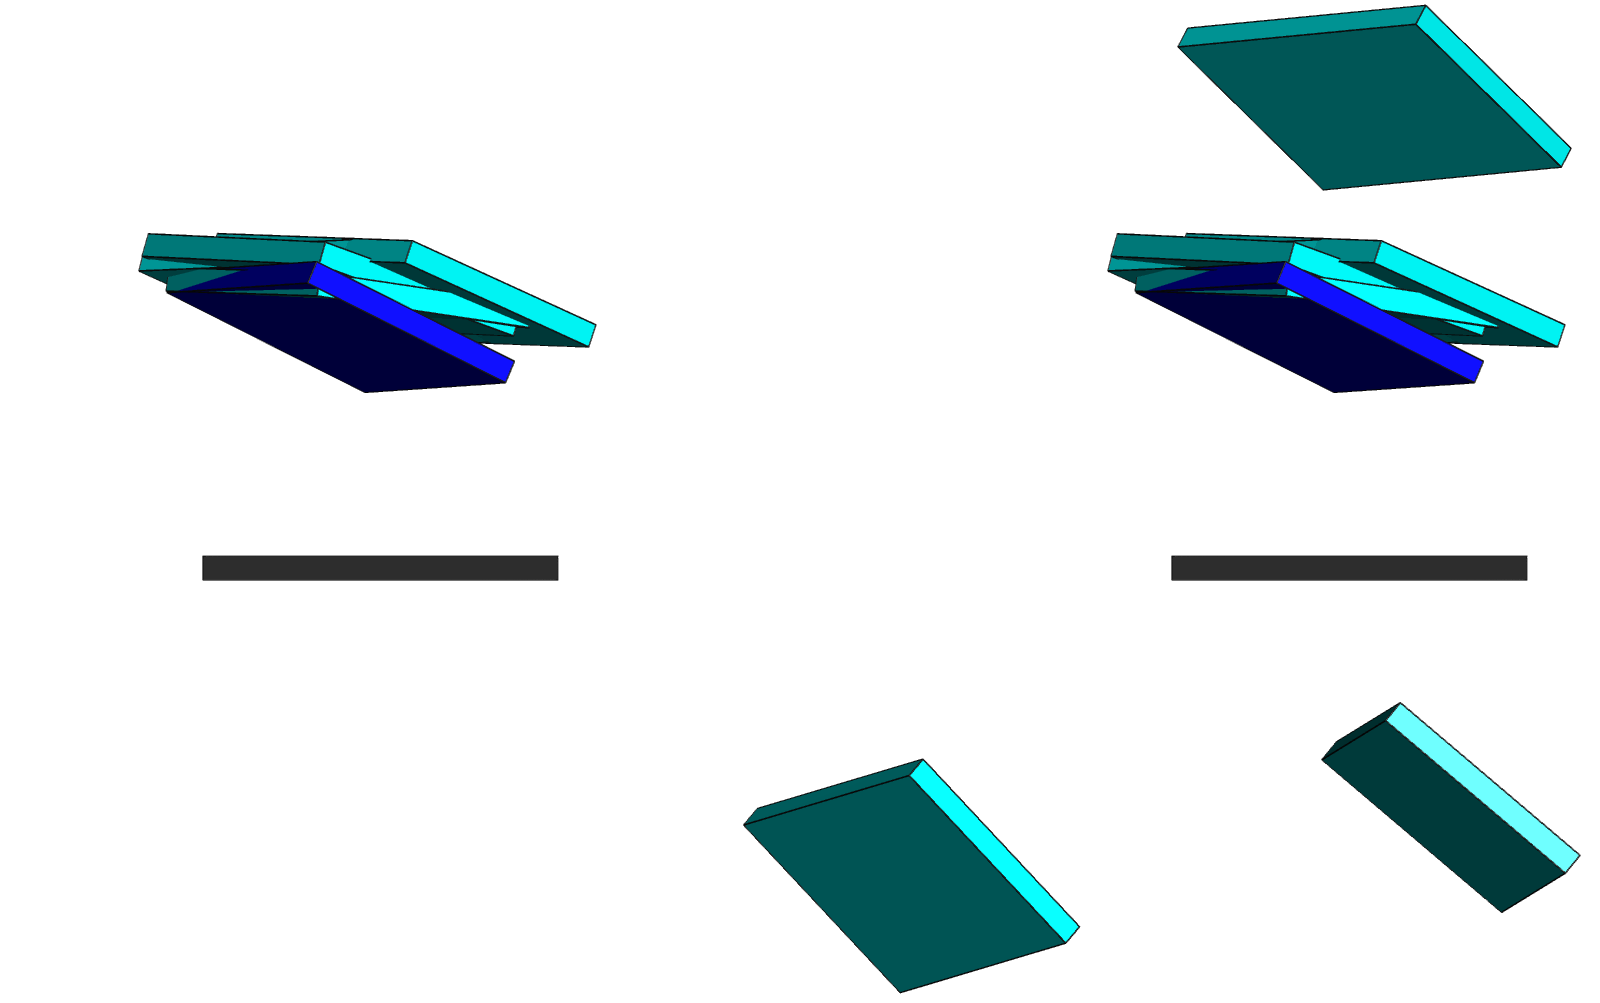
\includegraphics[angle=0, scale=0.3]{Chapter2/G1at10_15.png}
\caption{Rigid block  representation of dinucleotide  steps. The major
  groove side  of the first  nucleotide block is oriented  towards the
  viewer  and shaded  gray. \textbf{Left:}  Drawn in  blue,  the block
  representing       the        Group       I       cluster       from
  Figure~\ref{fig:nonAclus}. Superimposed  to the Group  I cluster are
  three  structures whose  step-parameter RMSD's  with respect  to the
  Group I  cluster are less than  or equal to  10 \AA. \textbf{Right}:
  With an RMSD less than or equal  to 15 \AA ~we "identify" a total of
  seven structures  from the  ribosome. We clearly  see that  three of
  them (encircled in  cyan blobs) are farther apart  from the original
  Group I  main structure of Figure~\ref{fig:nonAclus}  which is drawn
  in blue.}
 \label{fig:superimpose}
\end{figure}

\subsection{Selection of a Clustering Methodology} 
In  order to  analyze  our  dataset of  base-step  parameters we  have
decided  to  use  clustering  analysis methods.   Clustering  analysis
methods  can be broadly  classified into  two main  categories, either
partitional  or hierarchical.   In either  case the  main  problem one
faces for  classification purposes  is that of  deciding which  is the
optimal number of hierarchies or partitions that the analyzed data are
split into.  To obtain a  criterion for an optimal number of clusters,
and also  to decide which method  might be better for  our dataset, we
have used two types  of cluster-validation techniques.  They are known
as  internal measures  and stability  measures.  Full  details  of the
definitions  of   such  measures  are   provided  in  \cite{handl2005,
brock2008} and  Appendix~\ref{appendix_c}.  To perform  the validation
analysis  we   used  a  cluster  validation   package  called  clValid
\cite{brock2008},   which  is  implemented   in  the   R  \cite{rcite}
statistical analysis package.

In  Figures~\ref{fig:internal} and~\ref{fig:stability} we  present the
results  for  internal  and  stability  validation  of  the  base-step
parameters  in  the  23S  ribosomal  subunit.  In  clustering  anlysis
literature it is customary to use  a variable $k$ to define the number
of clusters.

We computed  the validation  scores for a  number of  clusters ranging
from  $k=2$, up  to $k=80$,  and evaluated  both  hierarchical methods
(hierarchical, diana)  and partitional (kmeans, pam,  som, sota).  The
connectivity  measure must  be minimized,  and the  average silhouette
width  (silhoutte) and  Dunn index  must be  maximized.  With  this in
mind,  we see  that the  hierarchical\footnote{The  hierarchical label
  refers  precisely to  the agglomerative  (bottom-up)  technique, the
  Euclidean metric, and the average method.} method performs better in
connectivity and  dunn index for the  whole range, and it  is also the
best performer in silhoutte from $k=12$ onwards.

Stability measures  (~\ref{fig:stability}) are well  suited for highly
correlated data sets with linear correlation between variables, but
they are not very useful for our data set,
which show  only such correlation in  shift and twist, as  can be seen
from  the values on  the upper  right corner  of the  pairs scatteplot
shown  in   Figure~\ref{fig:pairsnoarna}.   We  include   the  cluster
stability measures for completeness.

\begin{figure}
 \centering
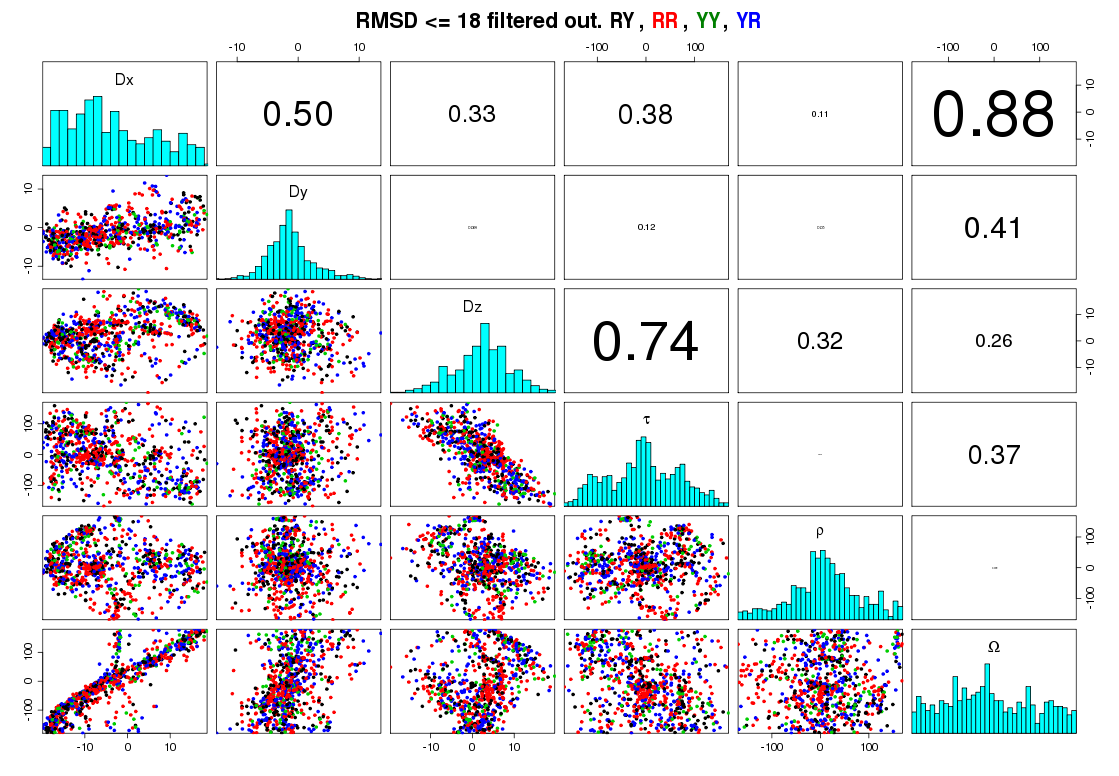
\includegraphics[angle=90, scale=0.5]{Chapter2/noarna_step.png}
\caption{Pairs  scatterplot for  base-step  parameters, shift,  slide,
rise,  tilt,  roll,  and  twist,  for the  non-A-RNA  dataset  colored
according   to   purine-pyrimidine   (black),   purine-purine   (red),
pyrimidine-pyrimidine    (green),    and   pyrimidine-purine    (blue)
steps. Here  the correlation coefficients of each  of the scatterplots
shown in the lower half of the graph are listed in the mirror position
in  the upper  half of  the  diagram, i.e.,  the shift-twist  ($D_{x},
\Omega$) correlation  coefficient (0.88) of the plotted  data shown in
the lower left corner, is printed in the upper right corner.}
 \label{fig:pairsnoarna}
\end{figure}

The stability measurements  we have computed are read  as being better
the smaller their values, of  these. We have determined three measures
for  each of  the hierarchical  and partitional  methods,  namely, the
average proportion  of non-overlap  (APN), the average  distance (AD),
and  the average  distance between  means (ADM).   The detail  of such
measures  is given  in Brock  et  al.  \cite{brock2008}.   As seen  in
Figure~\ref{fig:stability} the method with the best stability measures
is sota for APN  and ADM almost for the whole range,  up to ~ 70.  For
the AD  measure the best  performers are pam  and sota over  the whole
range.  Notice that the hierarchical  method follows the same trend as
the other methods, and that in general, apart from the APN measure and
the sota  method, all  methods exhibit a  similar behavior due  to the
fact that our data set is  not highly correlated. That is, the dataset
cannot be split into a few principal components.

In all cases  we also see that the best overall  number of clusters is
two, which is not surprising since we haven't filtered out A-RNA
structures from our  data set. The two main  groups are A-RNA
type base-steps, and non-A-RNA steps.

\begin{figure}
 \centering
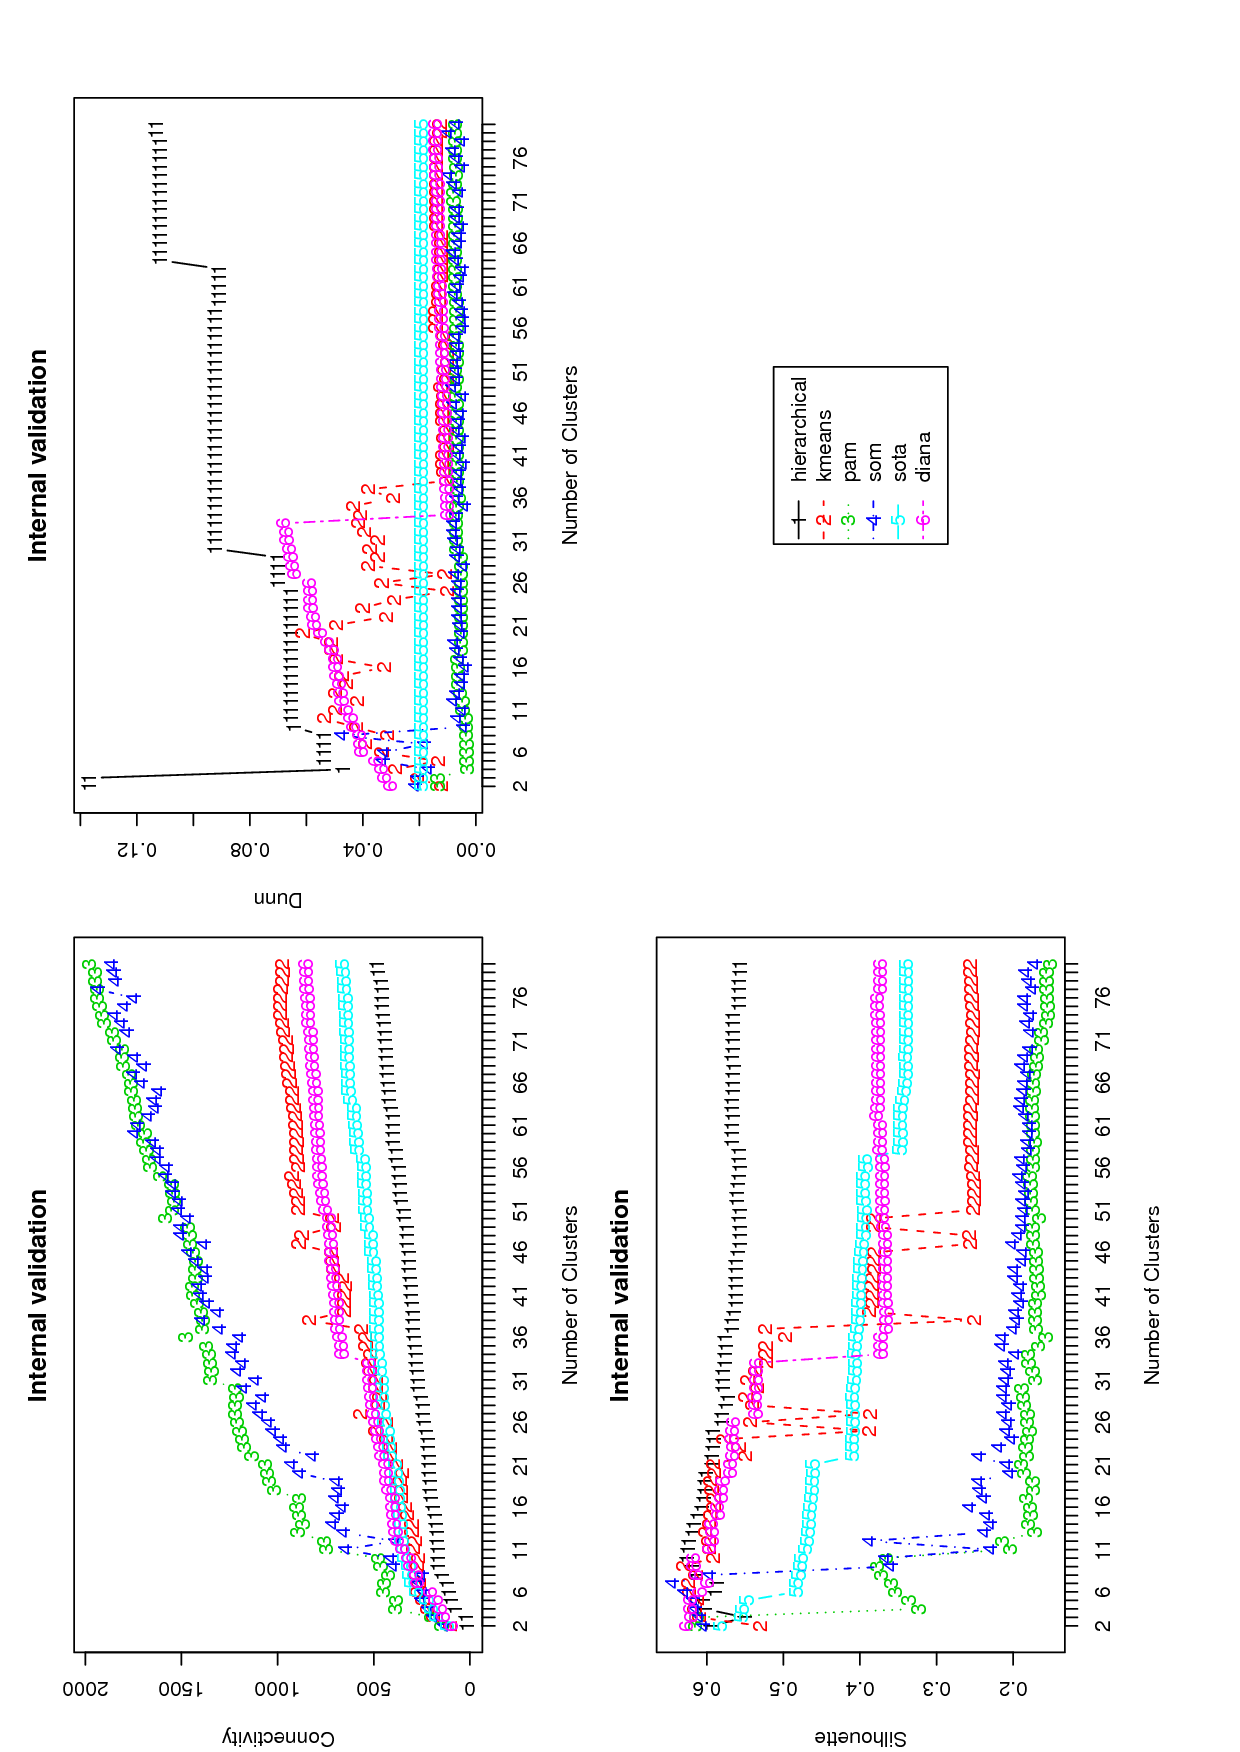
\includegraphics[angle=0, scale=0.38]{Chapter2/STval_int.png}
\caption{Cluster validity scores for internal measures. Notice how the
  hierarchical method, labeled as 1 in black color,
  behaves better for the whole range of Connectivity (smaller values)
  and Dunn (higher values),
  and it also outperforms all others after $k=12$ for Silhoutte
  (higher values) scores.}
 \label{fig:internal}
\end{figure}

\begin{figure}
 \centering
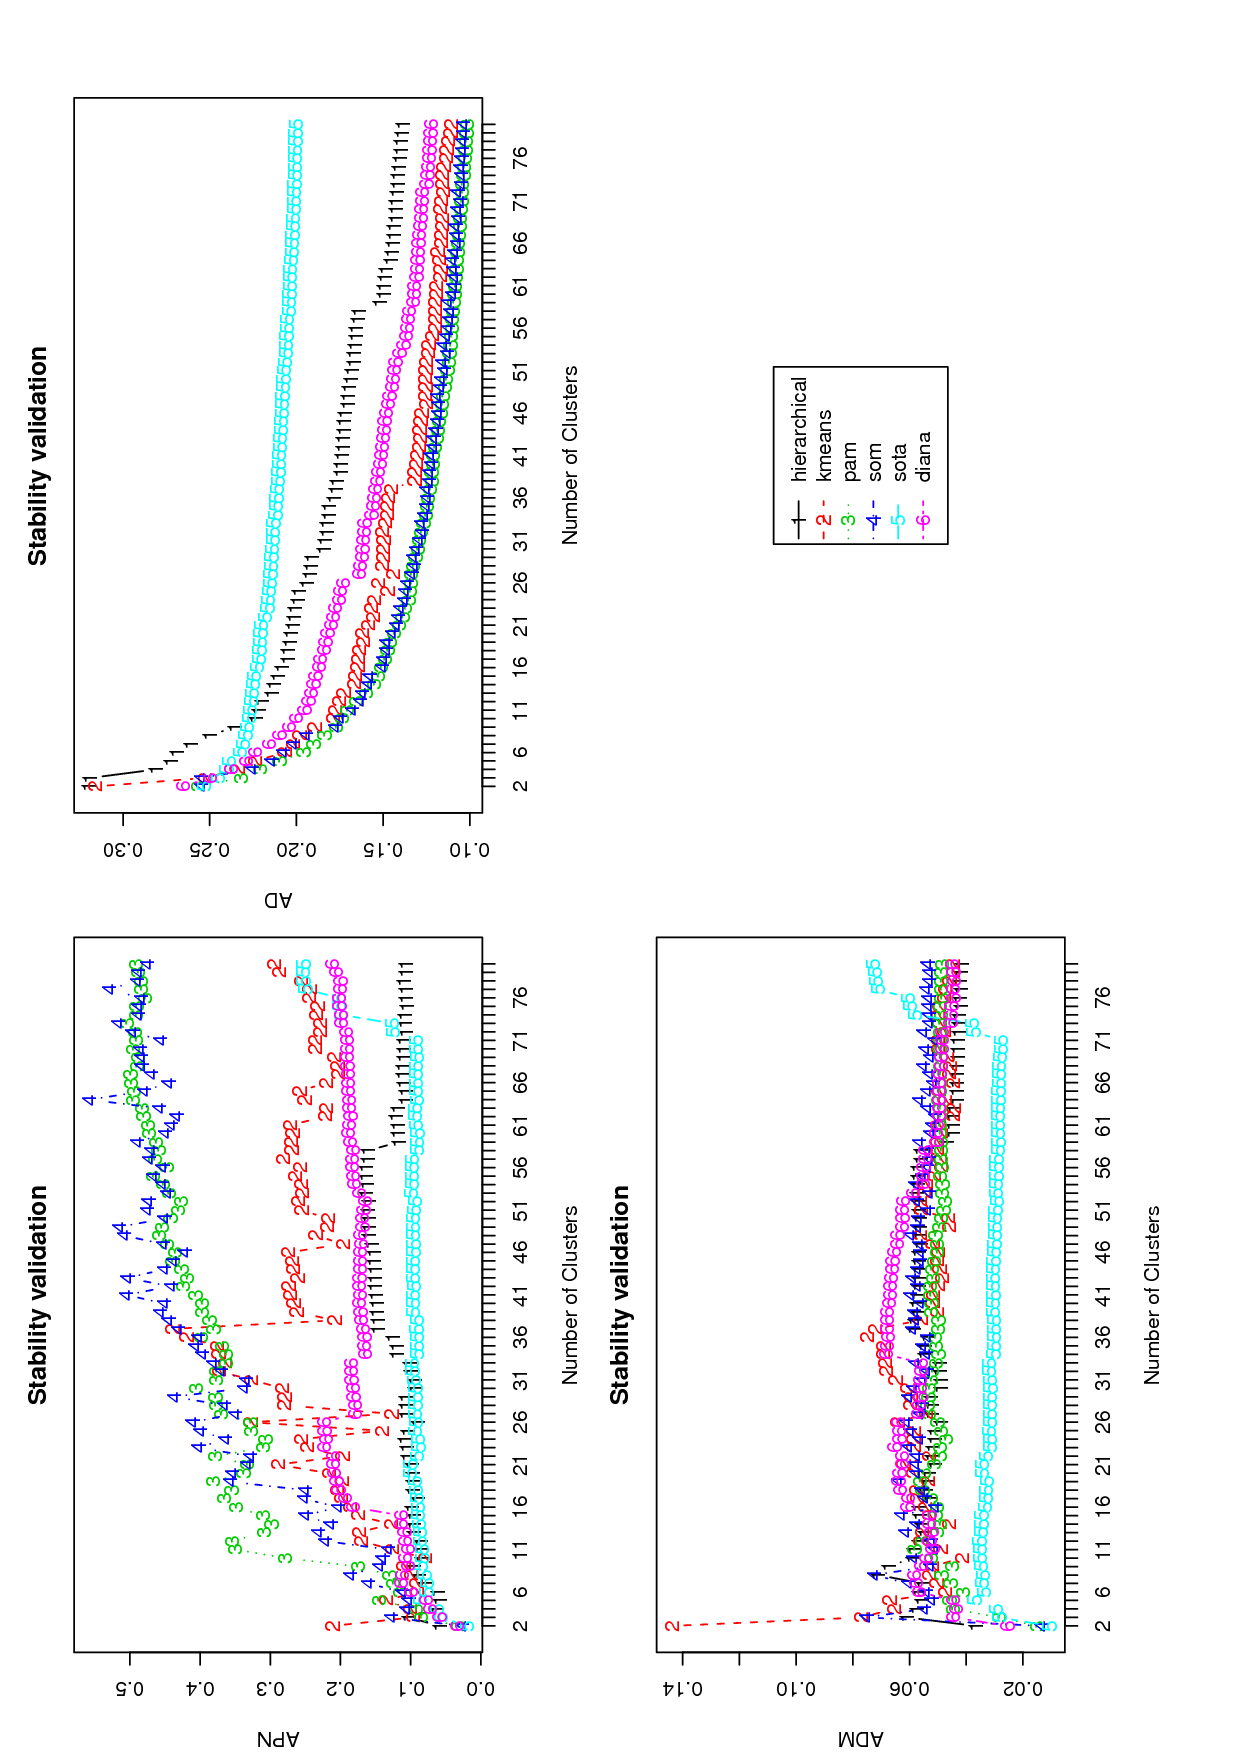
\includegraphics[angle=0, scale=0.38]{Chapter2/STval_sta.png}
\caption{Cluster validity scores for stability measures.}
 \label{fig:stability}
\end{figure}

We focus  our attention on the  group of structures  which differ from
A-RNA.  We have  extracted 797  such steps  (about 29\%  of  the total
number  of steps)  from  the  dataset based  on  the root-mean  square
deviation  between  step  parameters (Figure~\ref{fig:dormsd}).  These
base-step parameters are  those with RMSD values greater  than 18 \AA.
These RMSD values have  been computed between the base-step parameters
of  23S  RNA  and  the  standard base-step  parameter  values  of  the
canonical   A-RNA  helix  determined   by  Arnott   and  collaborators
\cite{arnott1973}  work. The standard  base-step parameter  values for
common    double-stranded    RNA     and    DNA    are    listed    in
Table~\ref{tab:conformations}.

\begin{figure}
 \centering
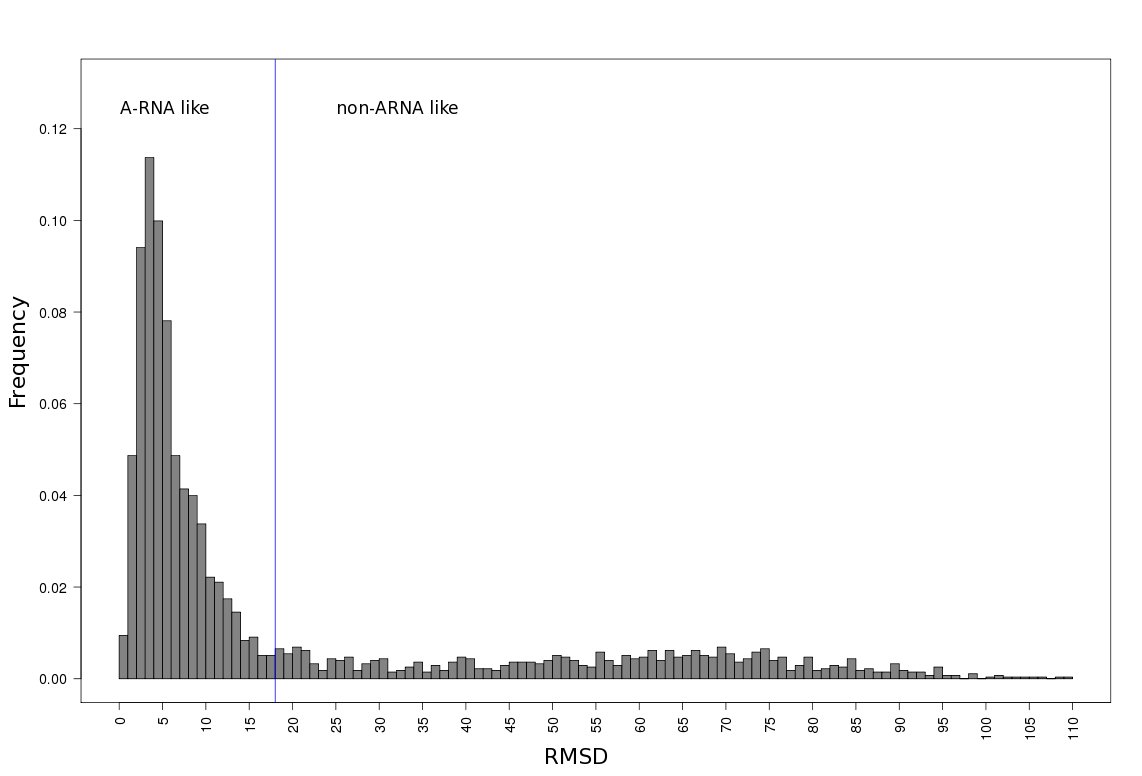
\includegraphics[angle=0, scale=0.3]{Chapter2/dormsd.png}
\caption{RMSD values between base-step parameters of the 23S subunit of
  ribosomal RNA and the standard base-step parameters derived from
  Arnott and collaborators \cite{arnott1973} work.}
 \label{fig:dormsd}
\end{figure}

\begin{table}
\begin{center}
{\small
\begin{tabular}{p{1.8cm}|c|c|c|c|c|c|c|c}
\hline
\textbf{Structure Name} & Shift ($D_x$) & Slide ($D_y$) & Rise ($D_z$) & Tilt
($\tau$) & Roll ($\rho$) & Twist ($\Omega$) & \textbf{Reference} &
\textbf{Method} \\ \hline
A-DNA & 0.36 & -1.39 & 3.29 & 2.46 & 12.50 & 30.19 & Arnott
\cite{arnott1999} & fiber-diffraction \\ \hline
B-DNA & 0.44 & 0.47 & 3.33 & 4.63 & 1.77 & 35.67   & Arnott
\cite{arnott1999} & fiber-diffraction \\ \hline
A-RNA & -0.08 & -1.48 & 3.30 & -0.43 & 8.64 & 31.57 & Arnott
\cite{arnott1999} & fiber-diffraction \\ \hline
A'-RNA & 0.05 & -1.88 & 3.39 & -0.12 & 5.43 & 29.52 & Arnott
\cite{arnott1999} & fiber-diffraction \\ \hline
AII-RNA & 1.01 & -2.52 & 3.33 & 2.94 & 9.75 & 25.12 & Schneider
\cite{schneider2004} & X-ray \\ \hline
\end{tabular}
}
\caption{Base step parameters for common DNA and RNA
  conformations. The base-step parameters are computed for
  a single-stranded base-step rather than a double-stranded base-pair step.}
\end{center}
\label{tab:conformations}
\end{table}

With the filtered dataset, which we refer to as the non-A-RNA dataset,
we  have repeated  the cluster  validation analysis  for  the internal
measures  (Figure~\ref{fig:noarna}). From this  analysis we  see again
that the  best method for  clustering our dataset is  the hierarchical
method. The Dunn index, which works under the idea of finding the best
possible separation  and compactness  between clusters, shows  us that
the optimal number of clusters  is $k=67$. The other two indices show,
as for the whole dataset case,  that the optimal number of clusters is
two, nonetheless, a common  indicative of optimal cluster solutions in
the  connectivity and  silhouette plots  is given  by the  presence of
shoulders.  We  see that there  is a shoulder  also at $k=67$  for the
connectivity and  silhouette plots. We selected the  67 clusters given
by   the   hierarchical   method,   and   took   their   corresponding
step-parameter values to  reconstruct the dinucleotide step structures
using 3DNA.  In Figure~\ref{fig:noarnak67} we draw the first seventeen
groups with  ten or more structures,  which account for  80 percent of
the  non-A-RNA steps.   We  also plot  in  the lower  right corner  of
Figure~\ref{fig:noarnak67} the  set of 20 structures  derived from the
work  of Schneider et  al.\cite{schneider2004}, and  the whole  set of
non-A-RNA  dinucleotide  steps in  a  common  reference  frame on  the
adenine  of  an ApU  step.   All  structures  are centered  using  the
standard  reference frame  embeded in  the  first base,  which in  our
reconstructions corresponds to a red block representing adenine, whose
minor groove  edge is oriented to  the left, its major  groove edge is
oriented  to the  right, and  its so-called  Watson-Crick base-pairing
edge is pointing towards the viewer.

When comparing the 17 groups of non-ARNA dinucleotide steps with those
coming from  the work  of Schneider and  collaborators we see  that in
their set  of structures there are  no steps represented  at the major
groove side of the red  block representing adenine, that is, the right
side of  the red adenine block. We  also see, that even  though the 17
groups represented are not as  compact as one would desire, they start
to  give an  indication of  geometrical  preferences on  the space  of
dinucleotide step-parameters.  For example, it is remarkable to see in
group  7, labeled  as  g7.png in  Figure~\ref{fig:noarnak67} that  the
blocks  representing  uracyl  in   cyan  color,  orient  their  planes
orthogonally to  the major groove  side of the red  block representing
adenine.

The reason we choose to  include the figure of all non-ARNA base-steps
in Figure~\ref{fig:noarnak67} is that of  giving the reader an idea of
the complexity of the  space of base-step conformations described from
a  base  viewed  perspective  instead  of  the  more  common  backbone
perspective, this also suggests that the task of finding order in this
broad range of possible conformations is analog to the task of peeling
an onion. We believe the onion can be effectively peeled into parts by
using  appropriate validated clustering  analysis techniques.

\begin{figure}
 \centering
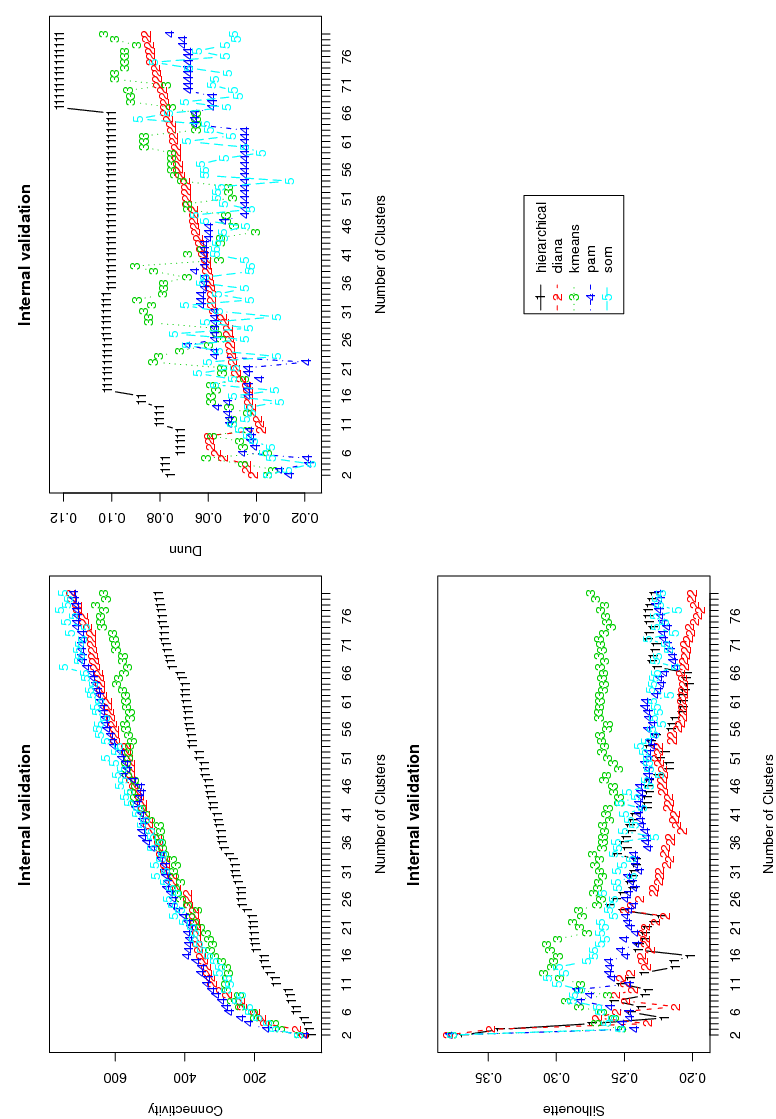
\includegraphics[angle=0, scale=0.9]{Chapter2/noarna_val.png}
\caption{Cluster validity  scores for the non-ARNA dataset.  It can be
  seen  clearly  that  the   optimal  method  for  clustering  is  the
  hierarchical one,  as measured by  lower values in  the connectivity
  scores, and higher  values in the Dunn score.  The optimal number of
  clusters given  by the dunn  score is 67,  we also see  shoulders at
  $k=67$, for the connectivity and silhouette scores.}
 \label{fig:noarna}
\end{figure}

\begin{figure}
\centering
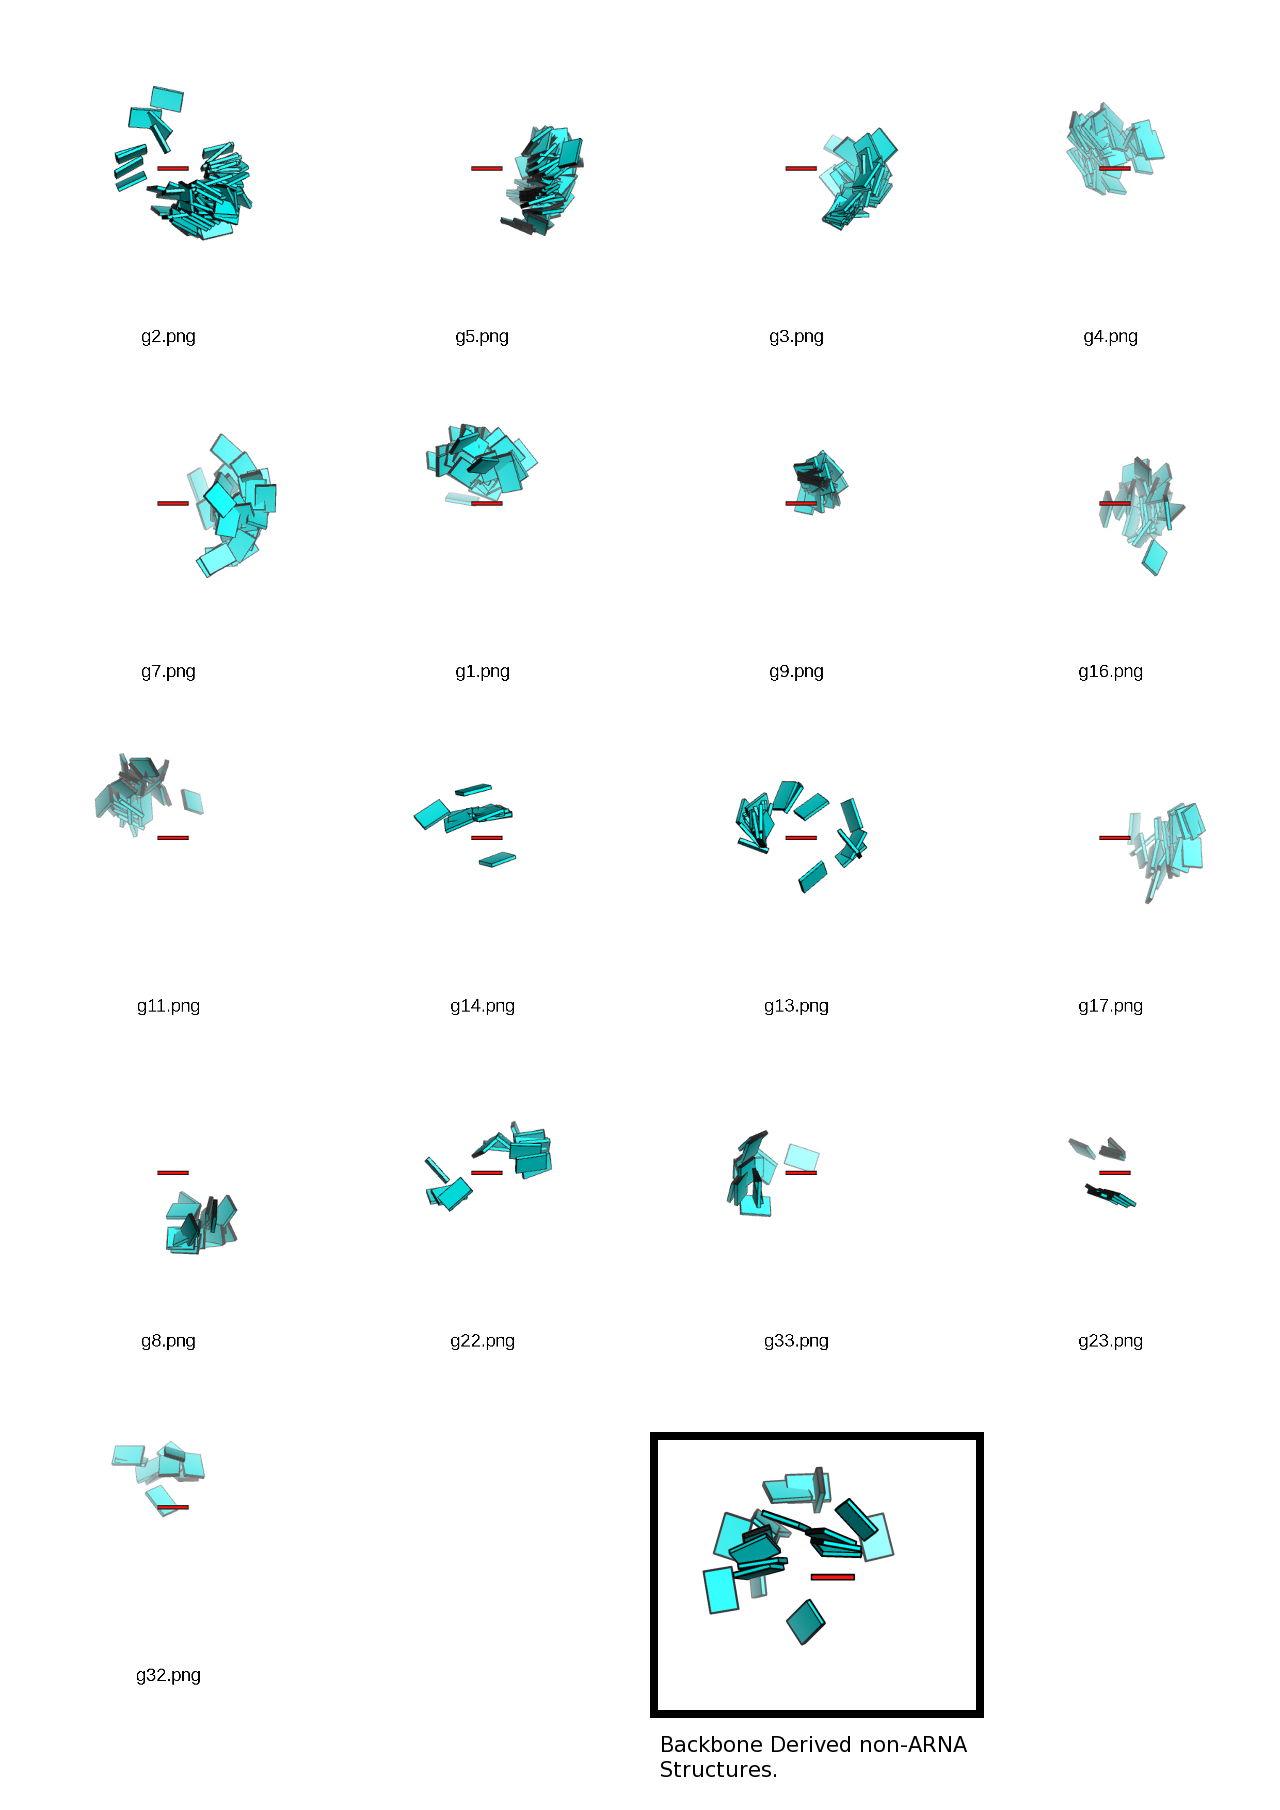
\includegraphics[angle=0, scale=0.35]{Chapter2/k67_17.png}
\caption{17  out of  the 67  groups clustered  using  the hierarchical
  clustering  algorithm  are  drawn  in  a  photograph  contact  sheet
  fashion. Each group  is centered on the base  reference frame of the
  adenine  block  drawn in  red.  In the  lower  right  corner of  the
  "contact sheet" the full space  of 797 reconstructed steps is shown,
  along with the  20 steps derived from schneider  et al. work. Notice
  how the only "hollow" side of the "onion" formed by the full space of
  base-step  conformations is that  corresponding to  the Watson-Crick
  base-pairing edge.}
\label{fig:noarnak67}
\end{figure}



\bibliography{biblio}

